\documentclass[10pt,a4paper]{article}
\usepackage[margin=14mm,top=11mm,bottom=11mm]{geometry}
\usepackage[T1]{fontenc}
\usepackage[utf8]{inputenc}
\usepackage{lmodern}
\usepackage{graphicx}
\usepackage{booktabs}
\usepackage{enumitem}
\usepackage{xcolor}
\usepackage{titlesec}
\usepackage[hidelinks]{hyperref}
\usepackage{microtype}
\usepackage{caption}
\captionsetup{font=small,labelfont=bf,skip=2pt}
\setlist{nosep,leftmargin=1.2em}
\titlespacing*{\section}{0pt}{5pt}{1pt}
\titleformat{\section}{\normalfont\normalsize\bfseries\color{teal!60!black}}{}{0pt}{}
\pagestyle{empty}

\begin{document}
\begin{center}
{\Large\bfseries Closing the Loop: Spec-Grounded, Self-Verifying AI Authoring of X3D 4.0 Scenes in the Browser}\\[3pt]
{\normalsize Technical overview of the \emph{X3D Copilot} prototype}\\[3pt]
\small Alberto Jaspe-Villanueva, King Abdullah University of Science and Technology (KAUST), \href{mailto:alberto.jaspe@kaust.edu.sa}{alberto.jaspe@kaust.edu.sa}\\[2pt]
\small Prototype: \url{https://albertojaspe.net/x3d-copilot/} \quad Source (MIT): \url{https://github.com/ajaspe/x3d-copilot}\\
\small\textit{Web3D 2026, AI \& Web3D Innovation Competition. Category: AI-Driven Content Generation.}\\[1pt]
\small\textbf{Live use:} the AI features require the user's own Gemini or Claude API key, entered in \textsf{Settings} (a free Gemini key from aistudio.google.com/apikey is sufficient); the key is stored in the browser and sent only to the provider. Editing, validation, the gizmo and import/export work without a key.
\end{center}

\section{Abstract}
Large language models produce X3D quickly, but their unassisted output is unreliable: invented field names, nodes placed in the wrong parent, malformed ROUTEs, mixed X3D versions, and no feedback about the rendered result. This prototype addresses the problem architecturally rather than through larger models or longer prompts. The model is grounded in the ISO/IEC 19775-1 X3D Unified Object Model, compiled into a database that it queries through a tool, and it can modify the scene only through validated edits. Each edit is checked against the official X3D~4.0 XML Schema, a semantic linter derived from the object model, and the X\_ITE runtime; the report is returned to the model, which repairs its own errors before answering. A screenshot tool lets the model inspect its own render. The approach yields AI-generated content that is standards-conformant by construction, inside a complete browser-based X3D editor with live rendering, direct manipulation and multi-format import, deployed as an open-source static site.

\begin{figure}[h]
\centering
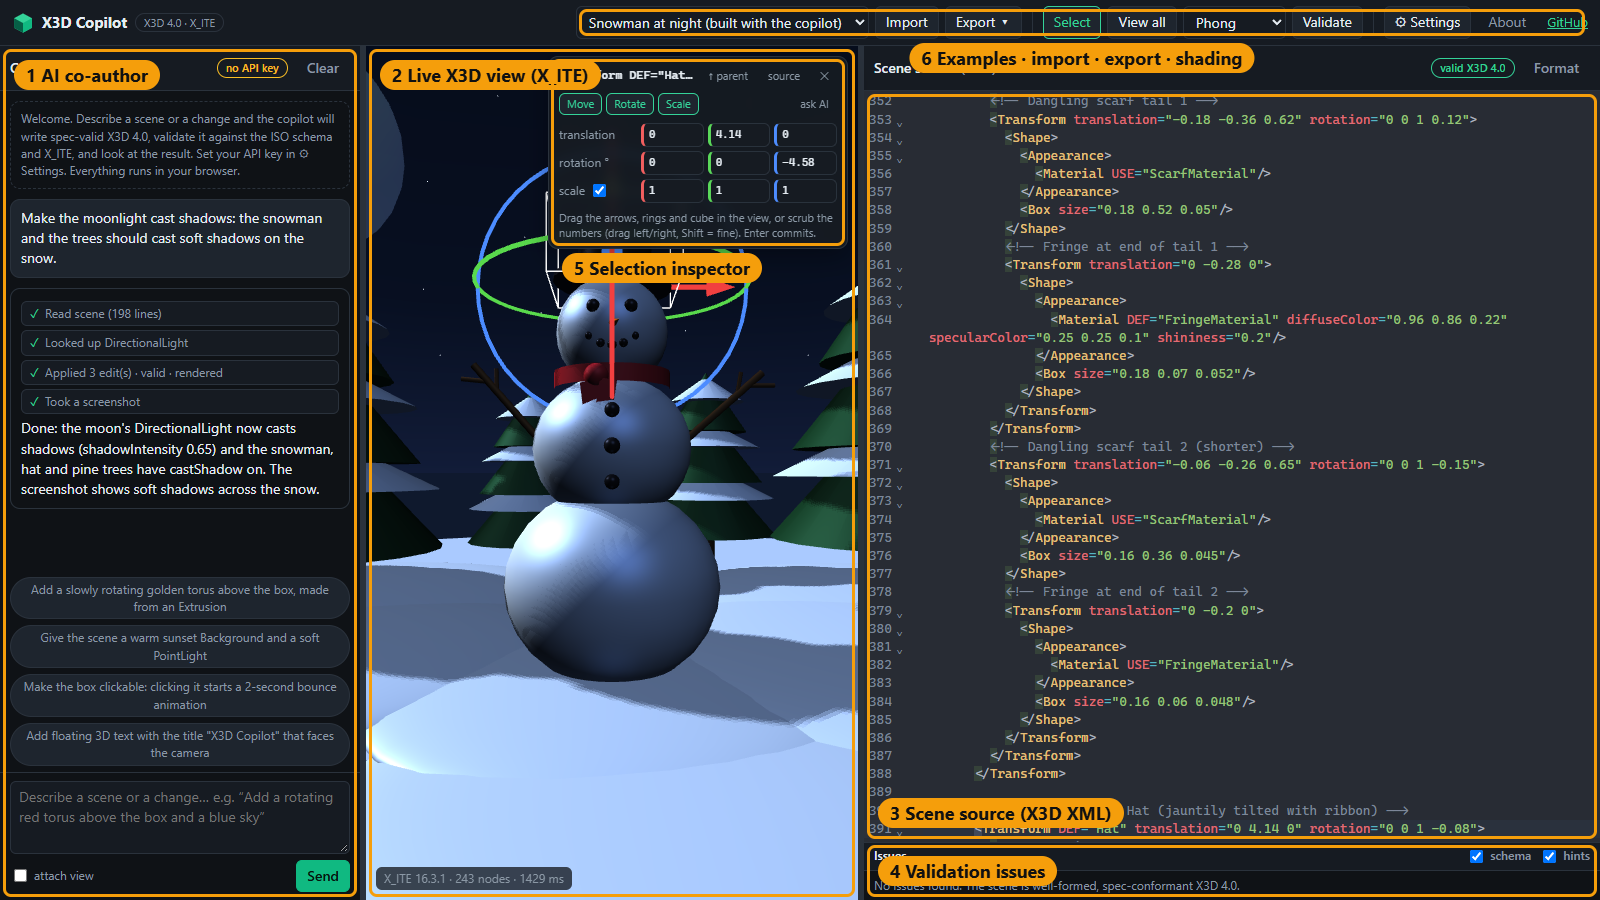
\includegraphics[width=0.96\textwidth]{fig-ui.png}
\caption{The interface, with the copilot-authored ``snowman'' example loaded and its hat selected. (1)~AI co-author: the conversation with the model; each tool call appears as a step (read scene, look up a node, apply edits, validate, screenshot) that can be expanded to show the validation report the model received. (2)~Live X3D view: X\_ITE~16 renders the scene as the source changes; clicking geometry selects its \texttt{Transform}, and the gizmo (arrows, rings, cube) is built from X3D \texttt{PlaneSensor} and \texttt{CylinderSensor} nodes injected at runtime. (3)~Scene source: a CodeMirror editor whose autocompletion (nodes, allowed children, fields with types and defaults) is generated from the X3D object model, with inline diagnostics. (4)~Validation issues: findings of the three validators, graded and attributed, with jump-to-line. (5)~Selection inspector: translation, rotation and scale of the selected node; edits are written back to the source as minimal attribute changes, and the selection is passed to the model as context. (6)~Toolbar: examples, import of glTF/OBJ/STL/PLY/VRML, export to X3D XML, Classic VRML, JSON and PNG, shading modes, model settings.}
\end{figure}

\section{AI integration}
\textbf{Models.} Google Gemini (3.8~Flash by default; 3.1~Pro and 2.5 selectable) and Anthropic Claude (Opus~5, Sonnet~5, Haiku~4.5) are accessed through their official JavaScript SDKs directly from the browser. A provider interface isolates each SDK in an adapter of about 150 lines, so the architecture is model-agnostic. Streaming, native function calling, images returned inside tool results, and effort or thinking controls are used where the provider supports them.

\textbf{Agent loop and tools.} The model never writes to the scene directly. A provider-neutral loop sends the system prompt, the tool definitions and the conversation, executes the returned tool calls locally, appends their results and repeats, up to 24 rounds per user turn. Seven tools are exposed: \texttt{get\_scene}; \texttt{edit\_scene} (exact, unique text replacements or anchored insertions; ambiguous edits are rejected); \texttt{replace\_scene}; \texttt{validate\_scene}; \texttt{lookup\_node} and \texttt{search\_nodes}, which return field definitions from the object model (type, accessType, default, accepted node types, containerField, component, specification URL) and flag nodes the running X\_ITE build does not implement; and \texttt{screenshot}, which returns the current frame as an image. Every scene-modifying tool returns the graded issue list with line numbers and the render status. The system prompt is short: it fixes the workflow (read before editing, prefer patches, resolve errors before answering, look up when unsure, screenshot when appearance matters) and a compact X3D~4.0 authoring guide. Correctness is enforced by the tools rather than by prompt text. A per-message note carries the user's current selection, so requests such as ``make this twice as big'' resolve to a specific node.

\section{Verification stack}
(1)~\textbf{Schema}: the official \texttt{x3d-4.0.xsd}, with the Web3D extension schemas and the W3C XML-Signature schema it imports, is vendored and compiled once by libxml2 running in WebAssembly; validation of a typical scene takes a few milliseconds. (2)~\textbf{Semantic linter}: about thirty rules that the schema cannot express, all driven by the object-model database: duplicate DEF, undefined USE, USE with a different node type, ROUTE to an unknown node or field, ROUTE from a non-output or to a non-input field, ROUTE type mismatch, a node in a parent field that does not accept it, several children in an SFNode field, attribute arity, type and range checks, zero rotation axes, interpolator key and keyValue consistency, empty groups, Shape without geometry, missing Viewpoint, and unknown nodes or fields with suggestions. (3)~\textbf{Runtime}: X\_ITE parse errors and console warnings are captured during load. Schema messages that duplicate a linter finding on the same line are demoted so that the model is not penalised twice. The three layers are independent modules sharing one issue format; the spec database is regenerated from the X3DUOM by a script.

\section{Web3D frameworks and standards}
X3D~4.0 (ISO/IEC 19775-1:2023) with its XML encoding (ISO/IEC 19776-1); the X3D Unified Object Model 4.0 (Web3D Consortium), compiled at build time into a database of 260 concrete nodes, 78 abstract types and 17 statements; X\_ITE~16.3 as rendering and runtime engine, including its glTF, OBJ, STL, PLY and SVG loaders and its XML, Classic VRML and JSON encoders (imports are normalised to X3D~4.0); CodeMirror~6 for the editor. All scenes produced by the tool are plain, portable \texttt{.x3d} files. The gizmo, the selection sensors and other runtime additions exist only in the X\_ITE scene graph and are never written to the user's file.

\section{User experience}
No installation is required. Natural-language authoring is combined with visible, expandable tool steps, so the user can always see what the model read, changed and verified. Direct manipulation uses an X3D-native gizmo and a numeric inspector, synchronised in both directions with the source; placing the text cursor on a node selects it in the view. Errors are phrased as actions, with suggestions and jump-to-line. Eight example scenes are included, among them one authored entirely through the copilot in four prompts (Figure~1) and a deliberately broken scene for exercising the repair loop.

\section{Novelty, impact and limitations}
To our knowledge, this is the first X3D authoring tool in which a language model (a)~reads node and field definitions from the ISO object model through a tool instead of relying on training memory, (b)~can act only through validated edits whose reports are returned to it, and (c)~inspects a screenshot of its own render before answering. The individual components are known; the contribution is their combination, which makes AI-generated X3D conformant by construction. Evidence is currently qualitative: in recorded sessions the model repaired a scene with eleven planted errors in one turn and built complete animated, interactive scenes (nested orbits, sensors, PBR materials, shadows, click behaviours) from short prompts; those scenes ship as examples. For the Web3D community, the tool lowers the entry barrier to X3D while raising conformance, which is relevant to education, rapid prototyping and the adoption of the standard. The pattern (machine-readable specification, validators as tools, visual check) transfers to glTF, USD or CityGML by exchanging the schema and object model. Deployment is a static site; the compute is the user's browser and their own model account. The project is open source under the MIT license, covered by 56 automated tests (schema fixtures, one test per linter rule, edit patching, gizmo mathematics, and a check that every example is lint-clean and schema-valid), with continuous integration on GitHub.

Limitations: selection targets \texttt{Transform} nodes only; the screenshot check is qualitative and the model's aesthetic judgement varies between runs; long generations depend on provider speed and quotas. Planned work includes HAnim-aware tools, glTF export through X\_ITE, retrieval over the X3D examples archive, and a quantitative evaluation of first-pass validity with and without the specification tools.

\begin{figure}[!b]
\centering
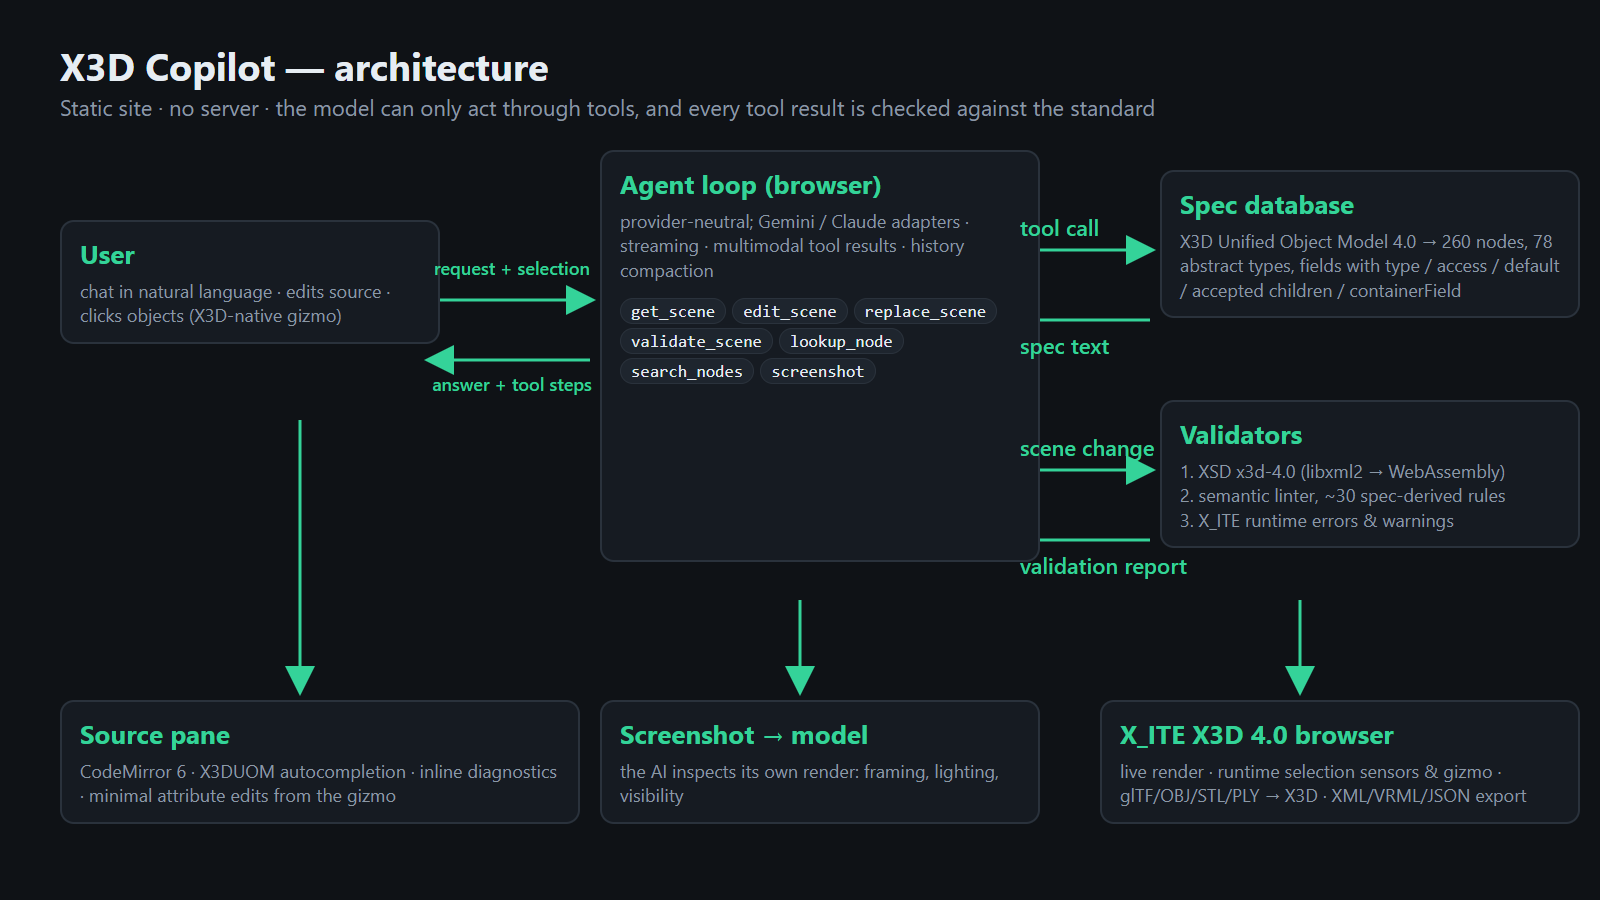
\includegraphics[width=0.44\textwidth]{architecture.png}
\caption{Architecture: the agent loop reaches the scene only through tools; the spec database answers lookups; validators and runtime grade every change; screenshots return the render to the model.}
\end{figure}
\end{document}
